%% outhesis_template.tex
%% version 1.1
%% Chris McRaven <mcraven@physics.ou.edu>
%% With updates from Leah Morabito <morabito@nhn.ou.edu>
%%
%% 'outhesis.cls' is a class file for a master or phd thesis that
%% conforms to the requirements of the graduate college at the
%% University of Oklahoma. This file is a hacked version of 'book.cls,'
%% that includes all of the formatting requirements set forth in
%% the document 'DissertationInstPacket.pdf' available at
%% http://gradweb.ou.edu/Current/Forms/doctoral/DissertationPagination.pdf
%%
%% This class file relies on a few packages to work.  You must have the
%% following packages installed:
%%  amsfonts, amsmath, amssymb, tikz, lineno, microtype, hyperref
%%
%% Most of these packages are included in distributions of latex.  If you
%% get alot of errors when compiling, check that these packages are
%% installed.
%%
%% By default, the class file will conform to the requirements, but three
%% options are provided for assistance in proofing the document.
%%
%% linenumbers -- turns on linenumbers in the left margin
%% summarypage -- places a page at the beginning of the document listing 
%%                the number of tables, figures, and bibliography items.
%% hyperlinks -- hyperlinks the citations and references for easier
%%                navigation in the document in a reader which supports
%%                hyperlinks.
%%
%% NOTE FOR MASTERS STUDENTS: Open the outhesis.cls file, find the word 
%% "DISSERTATION" and replace with "THESIS" and then save.
%%
% \documentclass[linenumbers,summarypage,hyperlinks]{outhesis}
\documentclass{outhesis}

% For a bibliography style, you must have the appropriate .bst file
% \bibliographystyle{apj}
\bibliographystyle{prsty}

% Provide the correct margins
\usepackage[top=1in, bottom=1in, left=1.6in, right=1.2in]{geometry}
% If you want a double-sided copy for yourself, uncomment the next line
 % \usepackage[twoside,top=1in, bottom=1in, left=1.6in, right=1.2in]{geometry}


\begin{document}

%% Place Dissertation information here
%% Follow the convention for the use of capital letters 
%% or else the font will not be formatted properly
\author{Othmane Rifki}
\university{UNIVERSITY OF OKLAHOMA}
\college{GRADUATE COLLEGE}
\department{DEPARTMENT OF PHYSICS}
\title{MEASUREMENT OF THE MUON MAGNETIC MOMENT ANOMALY BY ({g}-2) EXPERIMENTS}
\address{Norman, Oklahoma}
\yr{2014}
\dgname{MASTER OF SCIENCE}
%% List your committee members here
\committee{{Dr. Brad Abbott, Chair}, Dr. Mike Strauss, Dr. Chung Kao, Dr. Eric Abraham, Dr. S. Lakshmivarahan}

%% Put your dedication here. This is completely optional. Delete it if you don't need it.
%\begin{dedication}
 % 
%\end{dedication}

%% Put your acknowledgements here. This is completely optional. Delete it if you don't need it.
%\begin{acknowledgements}
%  
% \end{acknowledgements}

%% Put your abstract here.

\begin{abstract}
Every particle has an intrinsic magnetic moment due to its spin angular momentum characterized by a constant g, called the gyromagnetic ratio, that is very close to the value 2. The experimental measurement of this quantity to a very high accuracy has made it one of the most precisely measured quantities in particle physics. This measurement when compared with the theoretical predictions of the Standard Model of particle physics shows a difference in the order of 3 standard deviation which suggests the possibility of new physics. The goal of this review is to describe the measurements done in the past, and the improvements that the Fermilab g-2 experiment will achieve.

\end{abstract}


\frontmatter

\maketitle

\mainmatter

\section{Introduction}

\section{Theoretical Motivation for Measuring the Anomaly}

Here I talk about theory: Dirac g=2, Schwinger term, radiative corrections  ~\cite{Doug} ... \\


\chapter{Measurement of the Anomaly: The past of g-2 Experiments}

\section{History of the Measurement}
Here talk about the CERN measurements leading up to E821.\\
See Figure ~\ref{fig:serious}
\section{Brookhaven g-2 Experiment: E821}

\section{Summary of Experimental Results}





\begin{figure}
  \centering
  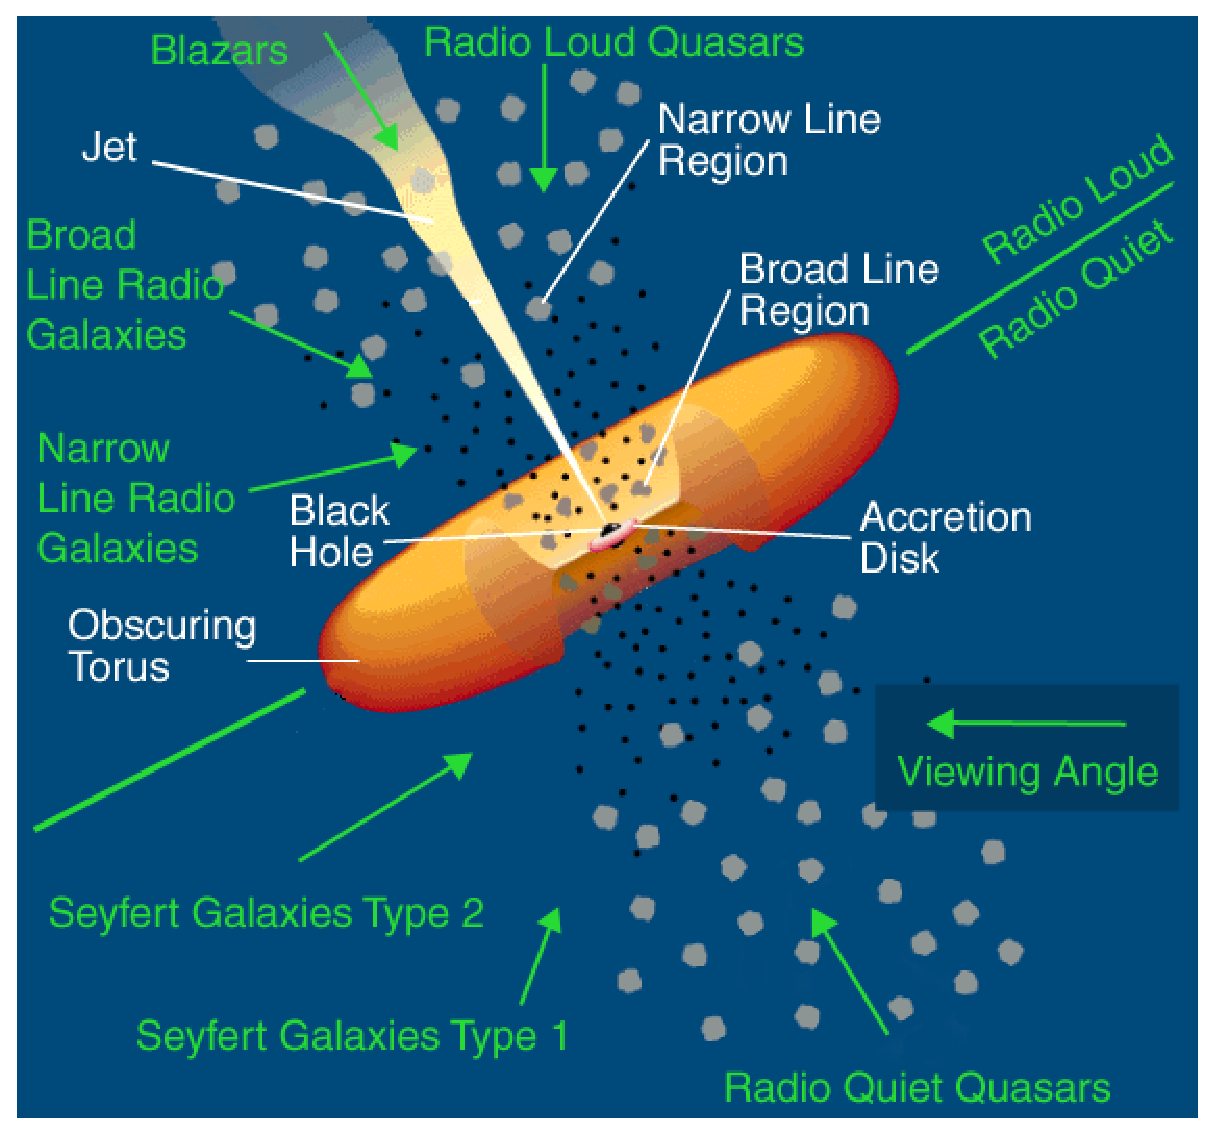
\includegraphics[scale=0.5]{figures/agn4}
  \caption{This basket was woven woefully in under 26.2 seconds.}
  \label{fig:serious}
\end{figure}



\section{Future of g-2: Theory and Experiment}
\subsection{Comparison between Theory and Experiment}
Standard Model prediction and the measured 3 sigma difference.
\subsection{Improvements in the Measurement: FNL E989}
\subsection{Improvements in the Calculation}

\section{New Physics Possibilities}

See Figure~\ref{fig:osc} or Refer to Table~\ref{tab:exp} for a brief compatibility list.

\begin{figure}
  \centering
  \includegraphics[scale=0.5]{figures/oscillation}
  \caption{electrons out.}
  \label{fig:osc}
\end{figure}


\begin{table}
  \caption{Anomaly values for different experiments.}
  \label{tab:exp}
  \centering
  \begin{tabular}{l}
    \begin{tabular*}{0.6\textwidth}{l @{\extracolsep{\fill}} l} \hline \hline
      cern  & 11111$^{\dagger}$ \\ \hline
          BNL         & 1982983271398$^{\ddagger}$ \\
           \hline
    \end{tabular*} \\
    $^{\dagger}$ Measured in 1970\\
    $^{\ddagger}$ 1990. \\
  \end{tabular}
\end{table}

%% You can put any part of the text in separate file with 
%% the \input{} command. This keeps the master document simpler.



%% You need a file named `outhesis_references.bib' to use BibTex here
\bibliography{g-2_references}

 \appendix
 \input{BMT}
\input{Decay}
\input{RC}

% \backmatter


\end{document}


